\documentclass{article}
\usepackage[margin=1in]{geometry}
\usepackage{amsmath, amssymb, bm, amsthm}
\usepackage{enumitem, hyperref}
\usepackage[breakable, skins]{tcolorbox}
\usepackage{graphicx}

\newtcolorbox{ans_box}[0]{arc=0mm, enhanced, frame hidden, breakable}

\setlength{\parindent}{0pt}
\setlength{\parskip}{0.5em}

\title{Exercises in Lie Theory}
\date{November 5, 2024}
\author{Rishav}

\begin{document}

\maketitle
\hrule
\tableofcontents
\newpage

\section{Topology}

\begin{enumerate}
  \item Give an example that in a general a family of open sets is not closed under infinite intersections.

  \begin{ans_box}
    Let us consider $\mathbb{R}$ under the metric d$(x,y)=|x-y|$ with open sets $U_{n}=\left(-\dfrac{1}{n},\dfrac{1}{n}\right)$.
    $$
    \bigcap_{n=1}^{\infty}U_{n}=\bigcap_{n=1}^{\infty}\left(-\dfrac{1}{n},\dfrac{1}{n}\right)=\{0\}
    $$

  Intersection of the open sets $U_{n}$ becomes narrower with increase in $n$ and approaches $\{0\}$ as $n\rightarrow\infty$.\medskip

  We know that a subset $U\subset\mathbb{R}$ is said to be open if, for every point $x\in U$, there exists an $\varepsilon>0$ such that the open ball $B(x,\varepsilon)=\{y\in\mathbb{R}\,|\,\text{d}(x,y)<\varepsilon\}$. We cannot create such open ball within a singleton $\{0\}$. Therefore $U_{n}$ is not closed under infinite intersection.
  \end{ans_box}

  \item Give an example that a bijective continuous function $f:E\rightarrow F$ between topological spaces is not necessarily a homeomorphism.

  \begin{ans_box}
    Let us consider that $E=\mathbb{R}$ has the standard topology generated by open intervals and $F=\mathbb{R}$ has the lower limit topology generated by basis of half-open intervals $[a,b)$ for $a<b$ where $a,b\in\mathbb{R}$. Furthermore, we define the function $f:E\rightarrow F$ as identity map i.e. $f(x)=x$.\medskip

  $f$, being an identity map, is clearly a bijection and also continuous because open sets in $E$ is also an open set in $F$. However, $f^{-1}:F\rightarrow E$ is not continuous because not every pre-image of open sets in $F$ is an open set in $E$ under $f$. For example, $[0,1)\in F$ is not an open set in $E$.
  \end{ans_box}

  \item Give an example of connected topological space which is not path connected.

  \begin{ans_box}
    Consider
    \begin{equation*}
      \begin{split}
        Y&=\{(0,y)\in\mathbb{R}^{2}|y\in[-1,1]\},\\
        Z&=\{(x,\sin\frac{\pi}{x})\in\mathbb{R}^{2}|x\in(0,1]\}, \text{ and}\\
        X&=Y\cup Z.
      \end{split}
    \end{equation*}

    Euclidean topology is induced on $X$ by inclusion on $\mathbb{R}^{2}$. \medskip

    $Z$ is connected space because it is an image of connected set $(0,1]$ under continuous sine function. $X$ is closure of $Z$ in $\mathbb{R}^{2}$ which makes $X$ a connected space. \medskip

    Let $\gamma:[0,1]\mapsto X$ be a path in $X$ that begins at $y\in Y$ and ends at $z\in Z$ with $\gamma(0)=y$ and $\gamma(1)=z$. Existence of such a map $\gamma$ would make $X$ a path-connected space. This can be contradicted if we show that $\gamma([0,1])\subseteq Y$ i.e. path is confined to $Y$.\medskip

    $\gamma^{-1}(Y)$ is certainly nonempty as it contains at least one element i.e. $0$. Suppose $t\in\gamma^{-1}(Y)$ and $\varepsilon>0$ with a value which ensure $\gamma\left((t-\varepsilon,\,t+\varepsilon)\right)$ is contained in a closed disc $D$ centered at $\gamma(t)$ and radius $r$. The intersection of this disc with $X$ consists of two intervals; i) closed interval in $Y$ and ii) closed segment of curve in $Z$ i.e. $$D\cup X=(D\cap Y)\cup(D\cap Z).$$

    We know that $(D\cap Y)\cap(D\cap Z)=\emptyset$, therefore $(D\cap Y)$ and $(D\cap Z)$ are separated from one another. Since $\gamma(t)\in D\cap Y$ and $(t-\varepsilon,\,t+\varepsilon)$ is connected, the image should be connected as well. This forces all the elements of $\gamma\left((t-\varepsilon,\,t+\varepsilon)\right)$ to be in $(D\cap Y)$ which implies $\gamma([0,1])\subseteq Y$.
  \end{ans_box}

\item  Give an example of a connected topological space which is not locally connected.

\begin{ans_box}
  Let us take connected space $X$ in above exercise. To show that $X$ is not locally connected, we have to find at least a point in $p\in X$ that does not contain a connected open neighborhood.

  Suppose an open disc centered on $p=(0,1)\in Y\in X$ with radius $r$. Since $Y$ is a closed set and $p$ is the edge of the line, there is no open connected open neighborhood of $p$.
\end{ans_box}

\item Recall the

  \textbf{Definition.} A topological space $X$ is \textit{totally disconnected} if the connected components of $X$ are single points.

  Give an example of a totally disconnected topological space.

  \begin{ans_box}
    Suppose $A=\{x\in\mathbb{Q}|x<\sqrt{2}\}=(-\infty,\sqrt{2})\cap\mathbb{Q}$ where the open segment $(-\infty,\sqrt{2})\in\mathbb{R}$ is open in $\mathbb{R}$ so $A$ is open in the subspace topology on $\mathbb{Q}$. Similarly $B=\{x\in\mathbb{Q}|x>\sqrt{2}\}=(\sqrt{2},+\infty,)\cap\mathbb{Q}$ is open in $\mathbb{Q}$ too. These open sets are disjoint and their union is $\mathbb{Q}$, therefore $\mathbb{Q}$ is not connected.\medskip

  Between any two rational numbers there exists an irrational number. Therefore $x,y\in\mathbb{Q}$ belong to different components of $\mathbb{Q}$. Indeed the components of $\mathbb{Q}$ are  singletons which, by definition, implies that $\mathbb{Q}$ is totally disconnected.
  \end{ans_box}
  \item Recall the

  \textbf{Definition.} Let $X$ be a topological space. A subset $S\subset X$ is said to be \textit{dense} in $X$ if, for each $x\in X$ and each neighborhood $U$ of $x$, there is a point $s\in S$ s.t. $s\in U$.

  Give an example of a dense subset of $\mathbb{R}$ (with usual topology.)

  \item Let $X$ be the space of continuous functions on the interval $I:=[0,1]$. Show that $$\text{d}(f,g):=\max_{x\in I}|f(x)-g(x)|$$ defines a metric on $X$.
\end{enumerate}

\section{Differential calculus}

\begin{enumerate}[start=9]
  \item Add to your personal mathematical tool box the following
  \paragraph{Definition.}

  \begin{enumerate}
    \item Let $E$ be a normed space and $f:U\subset E\rightarrow\mathbb{R}$ be differentiable so that D$f(u)\in L(E,\mathbb{R})=E^{*}$. In this case we sometimes write d$f(u)$ for D$f(u)$ and call d$f$ the \textit{differential} of $f$. Thus $\text{d}f:U\rightarrow E^{*}$.

    \begin{ans_box}
      \textit{What does it mean to compute derivative of real-valued function $f$ evaluated at point $u$? What kind of object is it?}\medskip

      $f$ is a linear map from a normed space to the field $\mathbb{R}$. Since the linear map is scalar-valued, it implies that $f$ is a \textit{linear functional}, also known as a \textit{covector}, which belongs to the \textit{dual space} of the normed space. By definition, the dual space is the set of all linear functionals on the normed space.\medskip

      In the real vector space $\mathbb{R}^{n}$, $E$ is typically considered as a set of column vectors, while an element of its dual space is a row vector. A row vector acting on a column vector yields a scalar in the field. This operation should not be confused with the inner product, since inner products are defined within the space itself, and the dual space is not directly involved. Furthermore, it is important to note that in finite-dimensional real vector space and its dual space are isomorphic.\medskip

      Usually in differential geometry, we often overlook partial derivatives because when a normed vector space is treated as a matrix space (which is also a vector space), complications arise when computing partial derivatives due to the two indices of the matrix. This is because computing partial derivatives with respect to both indices can lead to a more complex structure as we should differentiate with respect to both rows and columns simultaneously.  In contrast, in differential geometry, we often avoid these complications by using the language of \textit{differentials} and \textit{gradients}, which abstract away the need for explicit partial derivatives in cases like normed vector spaces. Instead of working directly with partial derivatives, we work with linear functionals and the dual space, which simplifies the process of differentiation in higher dimensions and more general spaces.\medskip

      $\text{d}f$ is a map that can be evaluated on an open subset $U$ of a normed space and yields an element in the dual space of that space i.e. it maps an space to its dual. $$\text{d}f:U\subset E\to E^{*}$$

      $\text{d}f(u)$ is a linear map that acts on a direction defined by an element of the domain, say $h$, and maps it to the corresponding directional derivative; $\text{d}f(u)\cdot h$. It is linear functional as it belongs to the dual space $E^{*}$, therefore, when applied to an element of vector space $E$, it produces an scalar. This is expressed as
      \begin{equation*}
        \begin{split}
          \text{d}f(u)&:E\to \mathbb{R}\\
          \text{d}f(u)&:h\mapsto \text{d}f(u)\cdot h\quad\text{where }u,h\in E.
        \end{split}
      \end{equation*}

    Clearly, $\text{d}f$ is different from $\text{d}f(u)$ because they are different maps. Though $\text{d}f(u)$ is a linear map, $\text{d}f$ is not itself linear. It is a family of linear maps parameterized by the point $u$. It is only when we evaluate $\text{d}f$ at a point, say $u$, do we get a linear map $\text{d}f(u)$. This is a crucial concept, and when thinking about derivatives, we should always ask ourselves, \textit{"What kind of mapping is it?"}.
    \end{ans_box}

    \item Let $(E, \langle.,.\rangle)$ be a Hilbert space and $f:U\subset E\rightarrow\mathbb{R}$ be differentiable. The \textit{gradient} of $f$ is the map grad$f=\nabla f:U\rightarrow E$ defined (implicitly) by $\langle\nabla f(u), e\rangle:=\text{d}f(u)\cdot e$, meaning the linear map d$f(u)$ applied to the vector $e$ (directional derivative).

    \begin{ans_box}
      $f$ is real-valued and differential of vector, as before, but with an added structure on the space i.e. it not just a normed space but the one with inner product.\medskip

      In the theory of ordinary differential equations (ODEs), there is a common idea that the gradient and the derivative are, in some sense, the same. However, this equivalence is generally \textit{not true}. The gradient is also not the transpose of the derivative (or differential); its definition depends heavily on the choice of the inner product. The notion of gradient from ODEs makes sense in $\mathbb{R}^{n}$ with the usual Euclidean inner product, where the dual space $(\mathbb{R}^{n})^{*}$ can be naturally identified with $\mathbb{R}^{n}$ due to isomorphism between them. In this specific case, the gradient aligns with the vector of partial derivatives. However, this is just a special case of a more general concept of the gradient, which does not apply universally.\medskip

    In the broader mathematical framework, different spaces often have different inner products. In such contexts, the ordinary concepts from calculus become awkward or insufficient, and the gradient must be redefined in terms of the specific inner product of the space. This highlights the importance of generalizing these notions beyond the classical Euclidean setting.\medskip

    The gradient of $f$, denoted $\nabla f$, is defined the unique vector field such that its dot product with any vector $e$ at each point $u$ is the directional derivative of $f$ along $e$. In other words, the inner product of $\nabla f$ evaluated at point $u$ with any vector $e$ is, by definition, the derivative of $f$ evaluated at $u$ in the direction $e$. i.e.
    $$
    \langle\nabla f(u), e\rangle:=\text{d}f(u)\cdot e
    $$
    $f$ being a differentiable function makes this relation well-defined.\medskip

    $u$ is a point in the space where the function $f$ is defined, and it represents the location where the gradient $\nabla f$ and the differential $df$ are evaluated. $e$ is a vector which represents a direction in which we measure the rate of change of the function $f$ at the point $u$.\medskip

    A Hilbert space has a non-degenerate inner product, and since we are dealing with a finite-dimensional space, the \textit{Riesz representation theorem} applies. This theorem implies that the linear functional $\text{d}f(u)\cdot e$, which represents the directional derivative of $f$ at $u$ in the direction $e$, can be expressed as the inner product of $e$ with a unique vector, denoted $\nabla f$. In this case, $\nabla f$ is the gradient. The non-degeneracy of the inner product ensures the uniqueness of $\nabla f$, making this a rigorous definition of the gradient.\medskip

    Expressing the gradient as a vector of partial derivatives, as is often done in engineering, can be misleading because it obscures the deeper relationship between the gradient and the inner product structure of the space. This inner product-based definition highlights the geometric and functional significance of the gradient.\medskip

    \paragraph{Relationship between gradient and derivative}
    The derivative is dual to the gradient. At each point, the derivative is a covector, a linear functional, or a cotangent vector that expresses how much the scalar output of a function $f$ changes with an infinitesimal change in the input vector in the vector space. The gradient at a point is a tangent vector that represents the direction and magnitude of the steepest infinitesimal change in the scalar output with respect to the vector input. The derivative is a map from the tangent space to the scalar field, while the gradient is an element of the tangent space at a point.\medskip

    In $\mathbb{R}^n$, $\nabla f$ and $\text{d}f$ are expressed as a column and a row vector respectively, with the same components but transpose of each other. Although they have the same components, they are different mathematical objects. i.e.

    \begin{equation*}
      \begin{split}
        \nabla f(p)&=
        \begin{bmatrix}
          \dfrac{\partial}{\partial x_{1}}(p)&\hdots&\dfrac{\partial}{\partial x_{n}}(p)
        \end{bmatrix}^{\top}\in\mathbb{R}^{n}\text{ and}\\
        \text{d}f(p)&=
        \begin{bmatrix}
          \dfrac{\partial}{\partial x_{1}}(p)&\hdots&\dfrac{\partial}{\partial x_{n}}(p)\\
        \end{bmatrix}\in(\mathbb{R}^{n})^{*}\\
        \implies\langle\nabla f(p), v\rangle&=\text{d}f(p)\cdot v=\dfrac{\partial}{\partial x_{1}}(p)+\hdots+\dfrac{\partial}{\partial x_{n}}(p)
      \end{split}
    \end{equation*}

    where $p,v\in\mathbb{R}^{n}$.
    \end{ans_box}
  \end{enumerate}

  \item

  \item Endow the vector space $\mathbb{R}^{n\times n}$ (matrix space) with the inner product $\langle A,B\rangle:=\text{tr}(A^{\top}B)$. Consider the smooth function $f:\text{GL}(\mathbb{R}^{n})\rightarrow\mathbb{R}$ defined by $X\mapsto\text{tr}(X^{-1})$ and compute grad$f(X)$.

  {\footnotesize Hint: Do not even try to work with partial derivatives.}

  \begin{ans_box}
    We are given a matrix space endowed with Euclidean or Forbenius inner product.
    \begin{equation*}
      \begin{split}
        \langle A,B\rangle&=\text{tr}(A^{\top}B)\\
        &=\sum_{i,j=1}^{n}a_{ji}b_{ji}
      \end{split}
    \end{equation*}

    It is an Euclidean inner product because, in principal, we can stack the column of $A$ and $B$ as a long vector $\tilde{A}$ and $\tilde{B}$. In doing so $\langle A,B\rangle$ is equal to the Euclidean norm of $\tilde{A}$ and $\tilde{B}$.\medskip

    $f:\text{GL}_{n}(\mathbb{R})\to R$ is a set of real invertible $n\times n$ matrices defined as $X\mapsto\text{tr}(X^{-1})$. $\text{GL}_{n}$ is an open and dense subset of a vector space $\mathbb{R}^{n\times n}$ because any $n\times n$ matrix can be arbitrary and accurately approximated by invertible matrix. i.e.
  $$
  f:\text{GL}_{n}(\mathbb{R})\subset\mathbb{R}^{n\times n}\to\mathbb{R}\\
  $$

  $\text{d}f$ is a mapping where we plug in invertible matrices and end up with a linear mapping $L$ which further maps the elements of the vector space to the reals. In other words, we evaluate the derivative of $f$ at a point in vector space, i.e. a matrix $X$, and we get linear functional $L$ where we can plug in direction $H$ (again a matrix in the vector space) to get an element in $\mathbb{R}$. $\text{d}f(X)$ takes direction and maps it to directional derivative. i.e.\medskip
  \begin{equation*}
    \begin{split}
      \text{d}f&:\text{GL}(\mathbb{R}^{n})\to L(\mathbb{R}^{n\times n},\mathbb{R}),\quad X\mapsto\text{d}f(x)\text{ and}\\
      \text{d}f(X)&:\mathbb{R}^{n\times n}\to \mathbb{R},\quad H\mapsto\text{d}f(x)\cdot H.
    \end{split}
  \end{equation*}

  Since we are dealing with a matrix space, trying to compute $\nabla f$ using partial derivatives is a no go. We must use the general definition of the gradient
    $$
    \langle\nabla f(X),H\rangle:=\text{d}f(X)\cdot H
    $$

  We will evaluate the right hand side of above equation and compare it with the left hand side to separate out $\nabla f$ using the given definition of the inner product.

  \begin{equation}
    \begin{split}
      \label{eqn:9a}
      \text{d}f(x)\cdot H&=\text{d}(\text{tr}(X^{-1}))\cdot H\\
      &=\text{d}(\text{tr}\circ X^{-1})\cdot H\\
      &=\text{d}(\text{tr})\circ\text{d}(X^{-1})\cdot H\\
      &=\text{tr}\circ\text{d}(X^{-1})\cdot H\\
      &=\text{tr}(\text{d}(X^{-1})\cdot H)
    \end{split}
  \end{equation}

  Above simplifications are made with following observations: The map $f$ is composition of taking inverse and trace. The derivative of composition of functions is composition of individual derivatives. The trace is linear and bounded so its derivative is equal to itself everywhere.\medskip

  Now we have to evaluate $\text{d}(X^{-1})\cdot H$. We know that invertible matrices fulfills $XX^{-1}=I$ independent of dimension where $I$ is identity in the space of $X$. We can take derivative of the expression in LHS along $H$ (directional derivative) using product rule for non commutative matrices. Derivative of LHS, a constant, is zero.
  \begin{equation}
    \begin{split}
      \label{eqn:9b}
      \text{d}(XX^{-1})\cdot H&=(\text{d}X\cdot H)X^{-1}+X\left(\text{d}(X^{-1})\cdot H\right)=0\\
      \implies\text{d}(X^{-1})\cdot H&=-X^{-1}(\text{d}X\cdot H)X^{-1}\\
      &=-X^{-1}HX^{-1}
    \end{split}
  \end{equation}

  We have utilized the fact that the derivative of $X$ is the identity mapping; $\text{d}X:X\mapsto X$. Consequently, the derivative of $X$ in the direction of $H$ is simply $H$ i.e. $\text{d}X\cdot H=H$.\medskip

  Finally, we substitute the the expression derived in Eqn.(\ref{eqn:9b}) into Eqn.(\ref{eqn:9a}) to compute $\nabla f(x)$. The cyclic invariance property of the trace, which results in $\text{tr}(ABC)=\text{tr}(CAB)=\text{tr}(BCA)$, is utilized to simplify the derivative.
  \begin{equation*}
    \begin{split}
      \text{d}f(x)\cdot H&=-\text{tr}(X^{-1}HX^{-1})\\
      &=-\text{tr}(X^{-2}H)\\
      &=\langle-(X^{-2})^{\top},H\rangle\quad\because\langle A,B\rangle=\text{tr}(A^{\top}B)\\
      \implies\nabla f(x)&=-(X^{-2})^{\top}
    \end{split}
  \end{equation*}

  In this exercise, we observe the potential danger of assuming that the gradient is simply the transpose of the differential, as is often done in $\mathbb{R}^{n}$. Here, such an assumption fails because we are working in a matrix space equipped with a different inner product, where the concept of a vector transpose does not directly apply.
  \end{ans_box}

  \item For $g:\mathbb{R}^{n\times n}\rightarrow\mathbb{R}^{n\times n}$, defined by $X\mapsto X^{3}$, for $H\in\mathbb{R}^{n\times n}$, compute the directional derivative D$g(X)\cdot H$.

  {\footnotesize Hint: Ditto.}

  \begin{ans_box}
    The function $g$ cubes the input square matrix, making it matrix-valued. Unlike the previous problem, we cannot leverage the cyclic invariance of the trace. In matrix spaces, multiplication is non-commutative, so expansions involving powers of $X$ must carefully preserve the order of terms. For instance, $g(A+B)=(A+B)^{3}$, which will be useful later in the computation, should be expanded using the distributive property while carefully preserving the order of multiplication.\medskip
    \begin{equation*}
      \begin{split}
        \label{eqn:12a}
        (A+B)^{3}&=(A+B)^{3}\\
        &=(A+B)(A+B)(A+B)\\
        &=(A+B)(A^{2}+AB+BA++B^{2})\\
        &=A^{3}+A^{2}B+ABA+AB^{2}+BA^{2}+BAB+B^{2}A+B^{3}
      \end{split}
    \end{equation*}

    To compute derivative, we perturb the argument in vector space linearly using a scalar parameter $\varepsilon$. We then take the derivative with respect to the $\varepsilon$, evaluated at $\varepsilon=0$. This process is called first order approximation.
  \begin{equation*}
    \begin{split}
      \text{d}g(x)\cdot H&:=\frac{\text{d}}{\text{d}\varepsilon}g(X+\varepsilon H)\bigg|_{\varepsilon=0}\\
      &=\frac{\text{d}}{\text{d}\varepsilon}(X+\varepsilon H)^{3}\bigg|_{\varepsilon=0}\\
      &=\frac{\text{d}}{\text{d}\varepsilon}X^{3}+\varepsilon X^{2}H+\varepsilon XHX+\varepsilon^{2} XH^{2}+
      \varepsilon HX^{2}+\varepsilon^{2}HXH+B^{2}X+\varepsilon^{3}H^{3}\bigg|_{\varepsilon=0}\\
      &=X^{2}H+XHX+HX^{2}
    \end{split}
  \end{equation*}
  \end{ans_box}

  Compute $\text{d}g(x)\cdot H$ using partial derivative for $\mathbb{R}^{2\times2}$ to get in touch with the contrast between the two methods.
\end{enumerate}

\section{Smooth manifolds}

\begin{enumerate}[start=13]
  \item
  \begin{enumerate}
    \item Consider the open subsets $U$ and $V$ of the unit circle $\mathbb{S}^{1}$ of $\mathbb{R}^{2}$ given by
    \item
    \item
    \item For $\mathbb{S}^{1}$ consider the \textit{stereographic projection} with x-axis image, i.e. $\{(U_{N},\varphi_{N}), (U_{S},\varphi_{S})\}$ with
    $$
    U_{N}:=\{(x,y)\in\mathbb{S}^{1}|y\neq1\},\quad U_{S}:=\{(x,y)\in\mathbb{S}^{1}|y\neq1\}
    $$

    Here $\varphi:U_{N}\to\mathbb{R}$ and $\varphi:U_{S}\to\mathbb{R}$ is given by
    $$
    \varphi_{N}:=\frac{x}{1-y},\quad\varphi_{S}(x,y):=\frac{x}{1+y}
    $$

    respectively. Prove that $\{(U_{N},\varphi_{N}),(U_{S},\varphi_{S})\}$ is a $\mathcal{C}^{\infty}$ on $\mathbb{S}^{1}$

    \begin{figure}
      \centering
      \label{fig:ex9}
      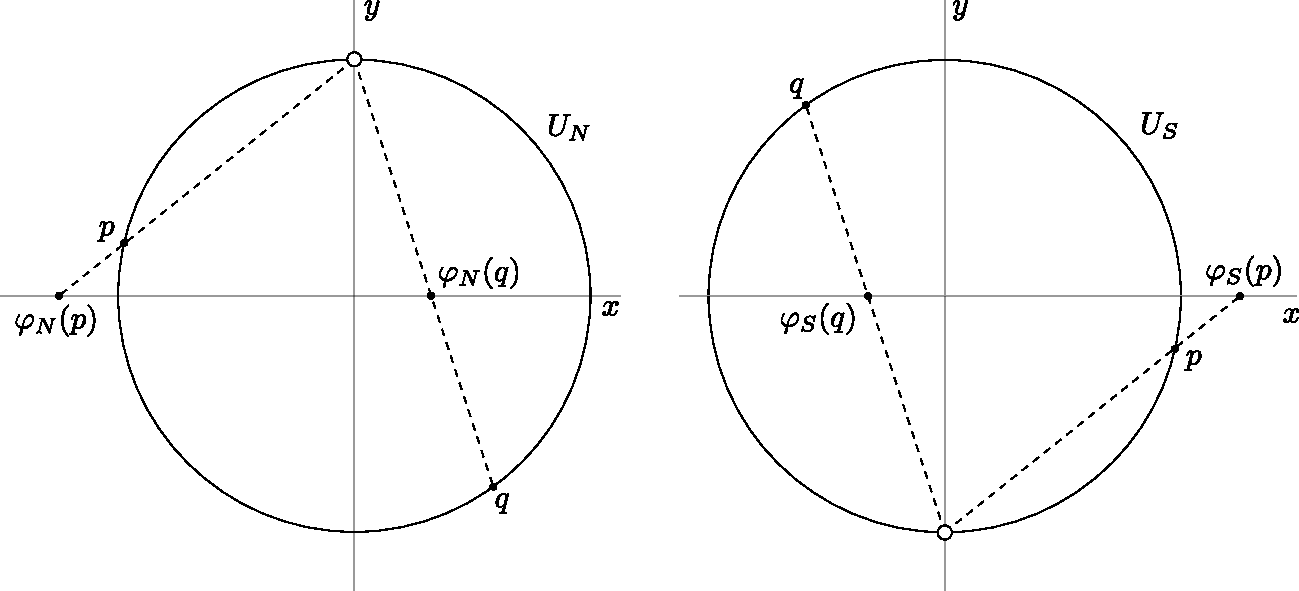
\includegraphics[scale=0.5]{assets/ex9.pdf}
      \caption{Stereographic projection of $\mathbb{S}^{1}$ into a x-axis.}
    \end{figure}

    \begin{ans_box}
      Intersection of straight line joining North (South) pole to any point $p$ on circle excluding the North (North) pole represents the projection of $p$ on the x-axis which is denoted by $\varphi_{N}(p)$. As the point $p$ approaches North pole, $\varphi_{N}(p)$ tends to either $+\infty$ or $-\infty$ as limit based on the direction of approach. Since the subset $U_{N}$ does not contain the North pole, the image of $\varphi_{N}$ is $\mathbb{R}\setminus\{-\infty,+\infty\}$ which is an open set.\medskip

      We have mappings from open subsets $U_{N}$ and $U_{S}$ of manifold $\mathbb{S}^{1}$ to an open subset of vector space which is homeomorphism. We can map whole of $U_{N}$ into the whole of x-axis ($\mathbb{R}$).  Its like spreading the ends of $U_{N}$ from the punctured North pole and stretching it over the x-axis. Same holds true for $U_{S}$. This is also the reason why (stereographic) maps on atlas is distorted as we move towards the poles. If we ever plan an expedition to the North pole, we should not carry the chart where North pole is not presented i.e. $U_{N}$. In such case, the map is distorted that moving a bit away from North pole takes us directly to the South. However, homeomorphism alone this is not enough to show that this is an atlas, or that these chart covers whole $\mathbb{S}^{1}$.\medskip

      If we have an atlas of Germany, one chart covers Bavaria and a bit of Baden-Württemberg. Similarly, next chart covers Baden-Württemberg something of Bavaria. This is done in such a way that such chart forms an atlas i.e. for any point on Germany, you are not stranded but are able to navigate through the country. In our case, we should be able to span whole space of $\mathbb{S}^{1}$ by switching the two charts. Mathematically, we have to show that the composition $\varphi_{N}\circ\varphi_{S}^{-1}$ is smooth. This suggests that, starting at any point on x-axis, we should be able to reach $U_{S}\in\mathbb{S}^{1}$ as governed by the map $\varphi_{S}^{-1}$ and back to the x-axis via the map $\varphi_{N}$. If this is not satisfied for all the points, we can conclude that these charts do not cover the entire circle.\medskip

      \textbf{Change of coordinates}\medskip

      Coordinates, by definition, are ways to express points on a manifold in terms of coordinates in open subset of the vector space. Therefore, we describe the points on $\mathbb{S}^{1}$ using the points the coordinate system of the real axis. We have to make sure there is intersection between charts; only then $\varphi_{N}\circ\varphi_{N}^{-1}$ is smooth.\medskip

      We have to evaluate $\varphi_{S}\circ\varphi_{N}^{-1}$, so let us evaluate $\varphi_{s}^{-1}$. We know that
      $$
      \varphi_{N}:p\mapsto\frac{x}{1-y}\quad\text{and}\quad x^{2}+y^{2}=1.
      $$

      Substitution leads us to
      \begin{equation*}
        \begin{split}
          x^{2}+y^{2}=1\\
          p^{2}(1-y)^{2}=1\\
          y^{2}(p^{2}+1)-2p^{2}y+(p^{2}-1)=0\\
          \implies y=\frac{2p^{2}\pm\sqrt{4p^{4}-4(p^{2}+1)(p^{2}-1)}}{2(p^{2}+1)}=\frac{p^{2}\pm1}{2(p^{2}+1)}.
        \end{split}
      \end{equation*}

      $y=1$ is directly rejected because we know that all the points of real line are not mapped to $y=1$.
      \begin{equation*}
        \therefore y=\frac{p^{2}-1}{p^{2}+1}\implies x=p\left(1-\frac{p^{2}-1}{p^{2}+1}\right)=\frac{2p}{p^{2}+1}
      \end{equation*}

      Finally, we can evauate
      \begin{equation*}
        \begin{split}
          \varphi_{S}\circ\varphi^{-1}_{N}&=\varphi_{S}\left(\varphi^{-1}(x,y)\right)\\
          &=\varphi_{S}\left(\varphi^{-1}\left(\frac{2p}{p^{2}+1},\frac{p^{2}-1}{p^{2}+1}\right)\right)\\
          &=\frac{1}{p}\quad p\in\mathbb{R}\slash\{0\}
        \end{split}
      \end{equation*}

      which is $\mathcal{C}^{\infty}$, and so is its inverse. Therefore, the charts are smooth on $\mathbb{S}^{1}$.
    \end{ans_box}

  \end{enumerate}
  \item
  \item
  \item \label{item:16} Show that the set GL$_{n}(\mathbb{R})$ of real invertible $n\times n$ matrices is a differentiable manifold.

  \item Similar to Exercise \ref{item:16} show that the set $\mathbb{R}^{n\times m}_{*}$, i.e., the set of all full rank real rectangular matrices with $n\leq m$ forms a $nm$-dimensional submanifold of the vector space $\mathbb{R}^{n\times m}\cong\mathbb{R}^{nm}$.
\end{enumerate}

\section{Tangent structures}

\begin{enumerate}[start=19]
  \item
  \item Let
  $$
  g:\mathbb{R}^{2}\rightarrow\mathbb{R}^{3},\quad
  \begin{bmatrix}x\\y\end{bmatrix}\mapsto
  \begin{bmatrix}x^{2}y+y^{2}\\x-2y^{3}\\ye^{x}\end{bmatrix}.
  $$

  \begin{enumerate}
    \item Compute $T_{\left[\begin{smallmatrix}x\\y\end{smallmatrix}\right]}g$ and $T_{\left[\begin{smallmatrix}0\\0\end{smallmatrix}\right]}g\cdot\left(4\dfrac{\partial}{\partial x}-\frac{\partial}{\partial y}\right)$ via the algebraic approach.
    \item Calculate the conditions that the constants $\lambda,\mu,\nu\in\mathbb{R}$ must satisfy for the vector
    $$
    \left(\lambda\frac{\partial}{\partial x}+\mu\frac{\partial}{\partial y}+\nu\frac{\partial}{\partial z}\right)
    \Bigg|_{g\left(\left[\begin{smallmatrix}0\\0\end{smallmatrix}\right]\right)}
    $$
    to be the image of some vector by $Tg$.
  \end{enumerate}

  \item Consider
  $$
  f:\mathbb{R}^{2}\rightarrow\mathbb{R},\quad
  \begin{bmatrix}x\\y\end{bmatrix}\mapsto
  x^{3}+xy+y^{3}+1.
  $$

  \begin{enumerate}
    \item Using the algebraic approach compute the tangent map
    $$
    Tf:T_{\left[\begin{smallmatrix}x\\y\end{smallmatrix}\right]}\mathbb{R}^{2}
    \rightarrow T_{f\left(\left[\begin{smallmatrix}x\\y\end{smallmatrix}\right]\right)}\mathbb{R}.
    $$

    \item Which of the points
    $p\in\left\{\begin{bmatrix}0\\0\end{bmatrix}, \begin{bmatrix}1/3\\1/3\end{bmatrix}, \begin{bmatrix}-1/3\\-1/3\end{bmatrix}\right\}$
    is $Tf$ injective or surjective at?
  \end{enumerate}

  \item Consider the smooth map
  $$
  f_{\theta}:\mathbb{R}^{2\times2}\rightarrow\mathbb{R}^{2\times2},\quad
  \begin{bmatrix}x&z\\y&t\end{bmatrix}=:X\mapsto A_{\theta}\cdot X,\quad\text{with}\quad A_{\theta}:=
  \begin{bmatrix}\cos\theta&-\sin\theta\\\sin\theta&\cos\theta\end{bmatrix}.
  $$

  \begin{enumerate}
    \item Compute the tangent map T$f_{\theta}$ via the algebraic approach.

    {\footnotesize Hint: It may be easier to proceed by first identifying $\mathbb{R}^{2\times2}\cong\mathbb{R}^{4}$ in a suitable way, but one certainly can go ahead without doing so, as well.}

    \item Compute $Tf_{\theta}V$ with
    $$
    V:=\cos\theta\frac{\partial}{\partial x}-\sin\theta\frac{\partial}{\partial y}+
    \cos\theta\frac{\partial}{\partial z}-\cos\theta\frac{\partial}{\partial t}.
    $$
  \end{enumerate}

  \item

  \item Consider the differentiable map
  $$
  \varphi:\mathbb{R}^{4}\rightarrow\mathbb{R}^{2},\quad
  \begin{bmatrix}x\\y\\z\\t\end{bmatrix}\mapsto
  \begin{bmatrix}x^{2}+y^{2}+z^{2}+t^{2}-1\\x^{2}+y^{2}+z^{2}+t^{2}-2y-2z+5\end{bmatrix}=:
  \begin{bmatrix}u\\v\end{bmatrix}
  $$

  \begin{enumerate}
    \item Find the (i) set of points of $\mathbb{R}^{4}$ where $\varphi$ is not a submersion, and (ii) its image.
    \item Compute a basis for ker$T\varphi\Big|_{[0\,1\,2\,0]^{\top}}$.
    \item Compute the image of the tangent vector $[0\,1\,2\,0]^{\top}\in T_{[0\,1\,2\,0]^{\top}}\mathbb{R^{4}}$ by the tangent of $\varphi$.
    \item Compute the image of the covector $(\text{d}u+2\text{d}v)\Big|_{\begin{smallmatrix}-1\\5\end{smallmatrix}}\in T^{*}_{\begin{smallmatrix}-1\\5\end{smallmatrix}}\mathbb{R}^{2}$ by the pull-back $\phi^{*}$, choosing point $\begin{bmatrix}0&0&0&0&0\end{bmatrix}^{\top}\in\varphi^{-1}\left\{\begin{bmatrix}-1\\5\end{bmatrix}\right\}.$
  \end{enumerate}

  \item Consider the differentiable map
  $$
  X:=xy\frac{\partial}{\partial x}+x^{2}\frac{\partial}{\partial z},\quad Y:=y\frac{\partial}{\partial y},
  $$
  and the map $f:\mathbb{R}^{3}\rightarrow\mathbb{R}$, defined by $f(x,y,z):=x^{2}y$. Compute the followings for $p=\begin{bmatrix}1\\1\\0\end{bmatrix}$

  \begin{enumerate}
    \item $[X,Y]\Big|_{p}$
    \item $[fX]\Big|_{p}$
    \item $(Xf)\Big|_{p}$
    \item $Tf\cdot X|_{p}$
  \end{enumerate}

\end{enumerate}

\section{Lie theory}

\end{document}